\subsection{Decomposing the Expected Forward KL}
\label{sec:sleep_details}
In this subsection, we decompose the expected forward KL objective $\mathcal{L}_{fwd}$ 
to obtain an unbiased stochastic gradient for stochastic gradient descent. 

First, observe that optimizing $\mathcal{L}_{fwd}$ does not require computing the intractable term $p(x)$:
\begin{align}
\argmax_\eta\; \mathcal{L}_{fwd}(\eta)
    & = \argmin_{\eta} \; \mathbb{E}_{x \sim p(x)}\Big[ \mathrm{KL}(p(z \mid x) \| q_\eta(z \mid x)\Big] \\
  &=\argmin_{\eta} \; \mathbb E_{p(x)}\Big[\mathbb E_{p(z \mid x)}\Big(\log p(z \mid x) - \log q_\eta(z \mid x) \Big)\Big]\\
%&=\argmin_{\eta} \; \mathbb E_{p(x)}\Big[\mathbb E_{p(z \mid x)}\Big( - \log q_\eta(z \mid x) \Big)\Big]\\
&=\argmin_{\eta} \; \mathbb E_{p(x, z)}\Big[- \log q_\eta(z \mid x) \Big]\label{eq:sleep_loss_simple}.
\end{align}
Notice the integrating distribution $p(x,z)$ does not depend on the optimization parameter $\eta$.
% In the ELBO, the integrating distribution is $q_\eta$, resulting in the need for reparameterization or other adjustments to compute stochastic gradients.
Thus, unbiased stochastic gradients can be obtained as
\begin{align}
    g = -\nabla_\eta \log q_\eta(z \mid x) \quad \text{ for } (x, z)\sim p(x, z).
\end{align}

In other words, at each iteration of SGD, we simulate complete data $(x,z)$ from the generative model and evaluate the loss $-\log q_\eta(z \mid x)$.
Here, ``complete data" refers to the image along with its catalog.
This loss encourages the neural network to map an image $x$ to a distribution $q_{\eta}(\cdot \mid x)$ that places large density on the image's catalog $z$.

We decompose the loss $-\log q_\eta(z \mid x)$ further.
Recall that $q_\eta$ fully factorizes over tile latent variables, and thus $-\log q_\eta(z \mid x)$ is a summation over all tile latent variables.
To evaluate $-\log q_\eta(z \mid x)$ for some $(x,z)\sim p$, first convert $z$ to its tile parameterization $(\tilde N^{(s,t)}, \tilde \ell^{(s,t)}, \tilde f^{(s,t)})_{s=1,t=1}^{(S,T)}$, as detailed in Appendix~\ref{sec:eval_var_distr}.
For each tile $(s,t)$, the variational distribution on the number of stars $\tilde N^{(s,t)}$ is categorical with probability vector $\omega^{(s,t)}\in\Delta^{N_{max}}$ (recall Section~\ref{sec:distr_on_tiles}).
The loss function for the number of stars becomes
\begin{align}
    - \log q_\eta(\tilde N^{(s,t)} \mid x) = -\sum_{n = 0}^{\tilde N_{max}} 1\{\tilde N^{(s,t)} = n\} \log \omega^{(s,t)}_n.
    \label{eq:cross_entropy_loss}
\end{align}
The vector $\omega^{(s,t)}$ is the output of the neural network, and \eqref{eq:cross_entropy_loss} is the usual cross-entropy loss for a multi-class classification problem.

Next, recall that in the variational distribution location coordinates are logit-normal and fluxes are log-normal.
Let $y$ generically denote either the logit-location or log-flux for a star in the sampled catalog $z$; let $(\hat\mu, \hat\sigma^2)$ be the Gaussian mean and variance returned by the neural network. Then the loss for these latent variables is,
\begin{align}
    -\log q_\eta(y \mid x) =
        \frac{1}{2\hat\sigma^2}(y - \hat\mu)^2
         + \frac{1}{2}\log(2\pi\hat\sigma^2).
         \label{eq:gaussian_sleep_loss}
\end{align}
The first term encourages network predictions $\hat\mu$ to be close to the sampled latent variable $y$, while $\hat\sigma^2$ encodes the uncertainty of the network: the second term encourages small uncertainties, but is
balanced by the scaling of the error $(y - \hat\mu)^2$ in the first term.

% By our discussion in Section~\ref{sec:factorization},
% only the $N = N^{(s,t)}$-th row of the triangular
% array of latent variables $\tilde \ell^{(s,t)}$ and $\tilde f^{(s,t)}$ needs to be evaluated. Therefore, the losses in the last two terms of~\eqref{eq:sleep_loss_decomp} are of the form
% \begin{align}
%     -\log q_\eta(y \mid x) = -\sum_{i = 1}^{\tilde N^{(s,t)}} \log q_\eta(y_{\tilde N^{(s,t)},i} \mid x).
% \end{align}

% To interpret~\eqref{eq:gaussian_sleep_loss}, observe that
% $y_{n,i}$ is the true (simulated) latent variable in the catalog and
% $\mu_{n,i}$ is the predicted value for that latent variable from the neural network.
% $\sigma_{n,i}$ is also outputted by the neural network, representing uncertainty -- the second term encourages small uncertainties, but this is
% balanced by the scaling of the error $(y_{n,i} - \mu_{n,i})^2$ in the first term.

The losses in~\eqref{eq:cross_entropy_loss} and~\eqref{eq:gaussian_sleep_loss} show that the
expected forward KL objective results in a supervised learning problem on complete data
sampled from our generative model:
the objective function for the number of stars is the usual cross-entropy loss for classification,
while the objective function for log-fluxes and logit-locations are $L_2$ losses in the mean parameters.


% In Section~\ref{sec:estep_sleep_compare}, we will see the benefits of using complete data and optimizing $q_\eta$ using the losses~\eqref{eq:cross_entropy_loss} and \eqref{eq:gaussian_sleep_loss}  rather than the traditional ELBO.

% \subsubsection{Reverse versus forward KL}
% \label{sec:kl_q_p}
% TODO: something about forward KL overestimates uncertainties, see Figure~\ref{fig:kl_q_p_schematic}.

% \begin{figure}[!ht]
%     \centering
%     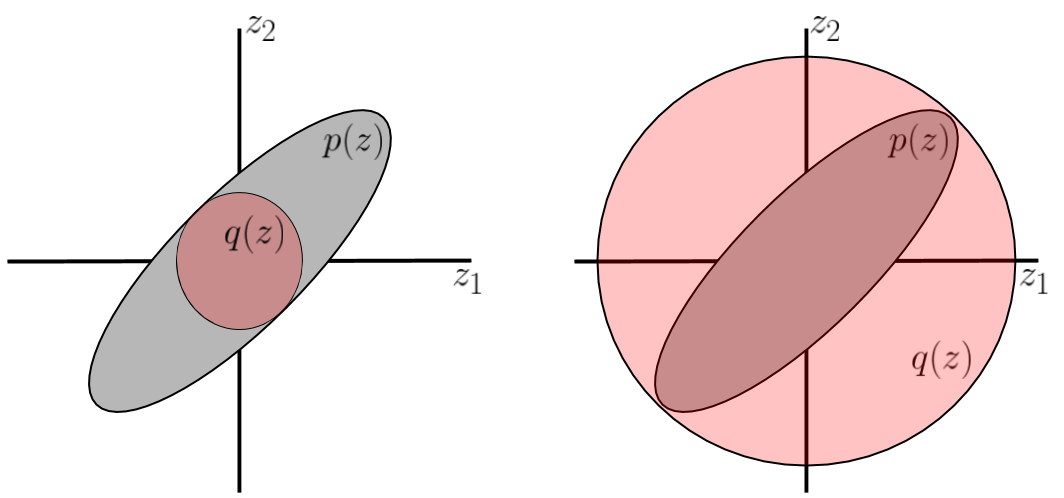
\includegraphics[width = 0.5\textwidth]{figures/kl_q_p_schematic.png}
%     \caption{A toy example where the target distribution $p$ is a bivariate Gaussian on
%     $z = (z_1, z_2)$ with positively correlated components.
%     $q$ is a mean-field variational approximation. Left, the optimal $q$ found
%     optimizing $\KL(q\|p)$; right, the optimal $q$ found optimizing $\KL(p\|q)$. }
%     \jeff{Are the contour lines for $p$ and $q$ the same (e.g., the contour that contains 50\% of the mass)? If so, is it true that these contours touch at exactly two point (rather than 0 or 4)? We should be correct on this detail if we're going to the trouble of showing a plot, even if we're just trying to get intuition.}
%     \label{fig:kl_q_p_schematic}
% \end{figure}
